%% LyX 1.3 created this file.  For more info, see http://www.lyx.org/.
%% Do not edit unless you really know what you are doing.
\documentclass[12pt,oneside,english]{book}
\usepackage[]{fontenc}
\usepackage[latin1]{inputenc}
\usepackage{geometry}
\geometry{verbose,letterpaper,tmargin=0.5in,bmargin=0.5in,lmargin=0.7in,rmargin=0.7in}
\usepackage{fancyhdr}
\pagestyle{fancy}
\setcounter{secnumdepth}{3}
\setcounter{tocdepth}{3}
\setlength\parskip{\medskipamount}
\setlength\parindent{0pt}
\usepackage{array}
\usepackage{longtable}
\usepackage{subfigure}
\usepackage{graphicx}

\makeatletter

%%%%%%%%%%%%%%%%%%%%%%%%%%%%%% LyX specific LaTeX commands.
\newcommand{\noun}[1]{\textsc{#1}}
%% Because html converters don't know tabularnewline
\providecommand{\tabularnewline}{\\}

%%%%%%%%%%%%%%%%%%%%%%%%%%%%%% User specified LaTeX commands.
\usepackage[bookmarksopen=true,pdftex]{hyperref}

\usepackage{babel}
\makeatother
\begin{document}

\title{Jumpshot-4's User's Guide}


\author{Anthony Chan%
\footnote{chan@mcs.anl.gov%
}, David Ashton%
\footnote{ashton@mcs.anl.gov%
}, Rusty Lusk%
\footnote{lusk@mcs.anl.gov%
}, William Gropp%
\footnote{gropp@mcs.anl.gov%
}\\
Mathematics and Computer Science Divsion, Argonne National Laboratory}

\maketitle

\section*{Acknowledgements}

One of the authors of this work, Anthony Chan, would like to thank
Dave Wootton of IBM Poughkeepsie for his valuable suggestions and
comments during the development of this tool. The software in this
work was in part developed by the DOE-supported ASCI/Alliance Center
for Astrophysical Thermonuclear Flashes at the University of Chicago.
This work was supported by the Mathematical, Information, and Computational
Sciences Division subprogram of the Office of Advanced Scientific
Computing Research, Office of Science, U.S. Department of Energy,
under Contract W-31-109-ENG-38.

\tableofcontents{}


\chapter{Introduction}

Jumpshot-4 is the visualization program for the improved scalable
logfile format, SLOG-2, which provides a hierarchical structure to
store a large number of drawable objects in a very scalable and efficient
way for visualization. The new scalable logfile format allows the
display program to provide functionalities never made possible before.
Level-of-detail support through preview drawables which provides high-level
abstraction of the details without reading in huge amount of data
into the graphical display engine. New Jumpshot allows seamless scrolling
from the begining till the end of logfile at any zoom-level. In addition,
new functionlities like dragged-zoom, grasp and scroll, instant zoom
in/out, easy vertical expansion of timeline, cut and paste of timelines
are available as well. A new search and scan facility is provided
to locate the hard-to-find objects in very large logfile. The new
legend table makes manipulation of the different category of objects
easy. The new viewer also attempts to conform to the standard Look
and Feel that is expected by most users.


\chapter{Data Model}


\section{Understanding the Drawable}

The main visual component in the SLOG-2 visualization program, Jumpshot-4,
is the \emph{timeline canvas} which is zoomable and scrollable in
both horizontal and vertical axes. The timeline canvas can be thought
of as a \noun{timeline} vs \noun{time} coordinate system. Each
point on the canvas is identified by two numbers, a timestamp and
a timeline ID. The canvas is where the graphical objects contained
in SLOG-2 file are being drawn on. These objects are called \emph{Drawables.}
There are 2 kinds of drawable objects. They are \emph{Primitive} and
\emph{Composite} drawables. The primitive drawables are the simplest
drawables and are considered to be basic elements of slog2 file. They
are categoried based on their topological structures. Currently, there
are 3 topologies supported in SLOG-2. They are \emph{State}, \emph{Arrow}
and \emph{Event}. Both state and arrow are drawables identified by
2 points in the timeline canvas, i.e. a pair of (timestamp, timelineID)
coordinates. State's start timeline ID is the same as its final timeline
ID, but arrow is different from state in the way that arrow's start
and final timeline IDs may be different. Event consists of only 1
point in the timeline canvas, i.e. it has only 1 timestamp and 1 timeline
ID. Composite drawable is more complicated and is constructed by a
collection of primitive drawables%
\footnote{In general, composite drawable can be seen as composed of other simpler
composite drawables.%
}. In order to centralize the properties of drawables, all the displayable
attributes of a drawable is stored in its corresponding \emph{Category}
object, e.g. color, legend name, topology and other shared description
of a drawable. Both the category and drawable definitions are stored
in the SLOG-2 file. These definitions are interpreted and displayed
by the display program, Jumpshot-4.


\section{Understanding the Preview Drawable}

A preview drawable is created as a result of the renormalization process
of the SLOG-2 format. The renormalized object provides a high-level
description of what is going on within the (timeline vs time) region
where the prevew object spans. Preview drawable is designed to amalgamate
real drawables of same topological type, e.g. preview state amalgamates
only states. So preview drawable is always a primitive drawable in
the renormalization scheme. There are currently 3 different types
of preview drawables: \emph{Preview\_State, Preview\_Arrow, and Preview\_Event.}
Therefore one preview drawable is for each supported topology of primitive
drawable. The three preview categories will always show up in the
Legend window of the display program as shown in Figure \ref{fig:legend_popup}
disregarding of the presence of preview drawables in the slog2 file.
The Legend window contains a table of legends. Each legend provides
an interface to the user modifiable part of the corresponding category
that is relevant to the display program. 

Figures \ref{fig:timeline_preview_detail_0} to \ref{fig:timeline_preview_detail_4}
illustrate the visual transition from preview drawable to its detailed
content of the first 5 processes of a 16 processes MPI slog2 file
when the timeline canvas is being zooming-in. The sequence of figures
is generated by zooming in a marked region in each figure in the sequence.
The marked region is shaded and is bounded by a pair of white lines.
A magnifying glass with plus sign in the center is the cursor that
marks the end of the zoom region. Figure \ref{fig:timeline_preview_detail_0}
is a typical timeline canvas where most of real drawables are still
buried by their preview drawables. In the figure, there are preview
arrows, preview states and some long running real states.

%
\begin{figure}[hbp]
\centering
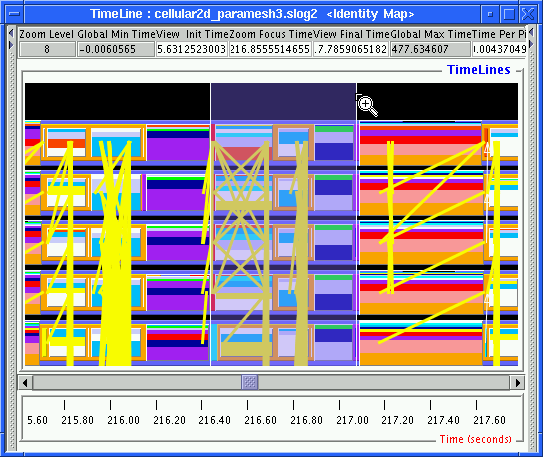
\includegraphics[%
  scale=0.6]{pic/timeline_preview_detail_0.png}


\caption{\label{fig:timeline_preview_detail_0} A typical zoom-out view of
preview states and arrows.}
\end{figure}


\noindent Each thick yellow line is a \emph{preview arrow} which represents
a collection of arrows between its 2 ending timelines. The start and
final timestamps of preview arrow are the extremes of all real arrows
amalgamated inside the preview object. Notice that the beginning or
ending timestamp of a preview arrow does not necessarily mean that
there is an arrow starting or ending at that time, it just indicates
that there are arrows starting and ending within these 2 times and
between the 2 marked timelines.

The rectangle that has horizontal strips of colors is \emph{preview
state}. The different colors inside a preview state represent the
various categories of real states that are amalgamated within the
time range of the preview state. Depending on the PREVIEW\_STATE\_DISPLAY
option selected in Preference window as shown in Figure \ref{fig:preference_pview_state}
and in Table \ref{table:preference_data2}, the distribution and the
heights of the strips can be changed as well. The default display
option for preview state is DECRE\_WEIGHT\_ORDER. In this option,
the strips are arranged in decreasing height order. The tallest strip
at the bottom of the preview state corresponds to the category of
states that contribute cumulatively the longest duration in specified
time range. This visual representation aims to tell what state categories
could be within the span of the preview state and which state category
contributes the most statistically to the specified time range, so
user can decide where to zoom in to find out more details. In a sense,
the preview states provide a global coarse-grain summary of what is
going on without losing as much details as the preview found in older
Jumpshot, i.e. Jumpshot-3. Compared with Jumpshot-3's preview which
has averaged out the timeline ID information, the new preview states
retain the timeline ID information and that may lead to early detection
of load balancing problem before zooming into seeing all the real
states. 

\noindent %
\begin{figure}[hbp]
\centering

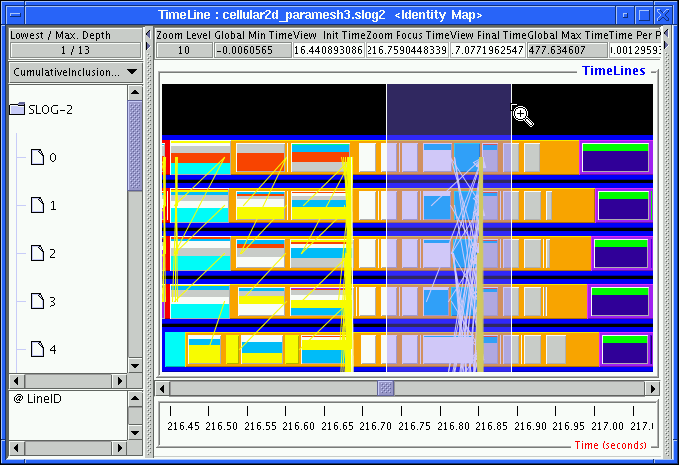
\includegraphics[%
  scale=0.6]{pic/timeline_preview_detail_1.png}


\caption{\label{fig:timeline_preview_detail_1} The next zoom-in view of Figure
\ref{fig:timeline_preview_detail_0}.}
\end{figure}


Figure \ref{fig:timeline_preview_detail_1} shows a more zoom-in view
of the region marked by the pair of white lines in Figure \ref{fig:timeline_preview_detail_0}.
As shown in Figure \ref{fig:timeline_preview_detail_1}, some of the
preview arrows have disappeared and are replaced by real arrows, the
white arrow. Also, some of the stripped preview states have split
into several preview states of one single color, i.e. the white and
grey states, to show more detailed distribution. Another important
feature of preview state becomes apparent in the figures: Preview
states are properly nested within real states. In the most expanded
Y-axis label view, preview state is always on top of other nested
states%
\footnote{Only in slog2 file that has multiple ViewMaps and where timelines
can be collapsed, i.e. AIX's UTE generated slog2 file, preview state
can be nested with other preview state in collapsed Y-axis label view.%
}, i.e. states that enclose the preview state are alway real states.
A good visual example is shown in Figure \ref{fig:timeline_preview_detail_1}
where all the white, turquoise and grey preview states%
\footnote{when a preview state contains only real states of one single category,
it will appear like a real state in the timeline canvas. The only
way to tell the difference is to bring up the Drawable Info Box by
right clicking on the state.%
} are sitting on top of the long orange and dark royal blue states.
This indicates that the white, turquoise and grey real states will
be all nested inside the long running orange and dark royal blue states.

%
\begin{figure}[hbp]
\centering

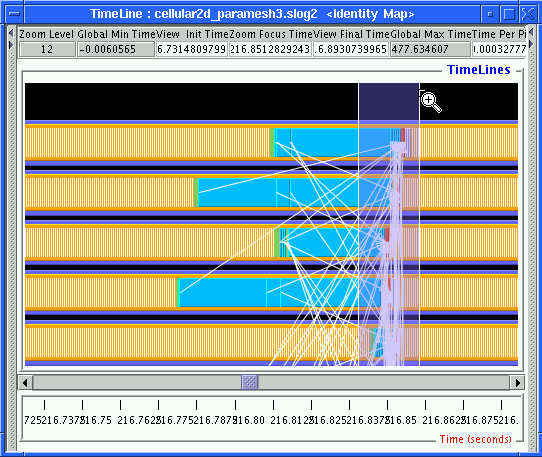
\includegraphics[%
  scale=0.6]{pic/timeline_preview_detail_2.png}


\caption{\label{fig:timeline_preview_detail_2} The next zoom-in view of Figure
\ref{fig:timeline_preview_detail_1}.}
\end{figure}


Figure \ref{fig:timeline_preview_detail_2} is the zoom-in view of
the region marked by the pair of white lines in Figure \ref{fig:timeline_preview_detail_1}.
Comparing these 2 figures, all the preview drawables have disappeared
and are replaced by real drawables. Each white preview state are repleaced
by hundreds of white real states, the same is also true for the grey
preview states that sit to the right of the turquoise states%
\footnote{In order to speed up grahics performance of the display program, an
aggressive algorithm has been employed to eliminate drawing states
that are closely packed together within the nearest neighboring pixels.
Together with the fact that the number of pixels available is less
than the number of non-overlap states in the region, the number of
the real states may sometimes not appear as numerous as the Drawable
Info Box of preview state indicates. In that case, a further zoom
in will be needed to confirm the case as shown in Fig. \ref{fig:timeline_preview_detail_3}.%
}. The preview arrows are all replaced by the real arrows. It becomes
apparent that the white lines marked region in Figure \ref{fig:timeline_preview_detail_1}
provides a good description of what is going on in Figure \ref{fig:timeline_preview_detail_2}
but at the same time it reduces the number of drawables drawn on the
canvas by a factor of 100. Another way of seeing this benefit is to
find out the exact number of real drawables amalgamated by the preview
objects within the zoomed region. This can be achieved by right clicking
on the preview drawable and the result is shown in Figure \ref{fig:timeline_infobox_preview_state}.

%
\begin{figure}[hbp]
\centering

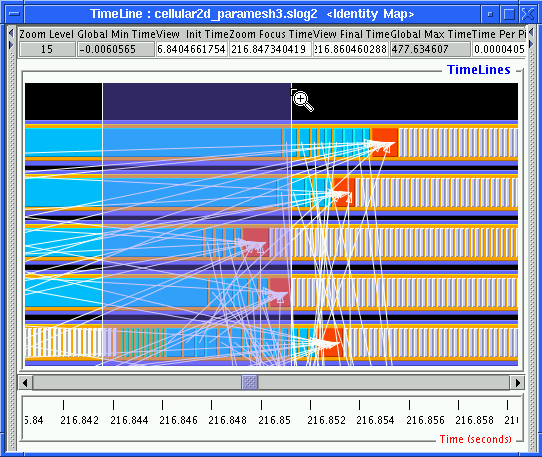
\includegraphics[%
  scale=0.6]{pic/timeline_preview_detail_3.png}


\caption{\label{fig:timeline_preview_detail_3} The next zoom-in view of Figure
\ref{fig:timeline_preview_detail_2}.}
\end{figure}


Further zooming into the white lines marked region in Figure \ref{fig:timeline_preview_detail_2}
enlarges the real drawables that are displayed in the figure. The
enlarged view is shown in Figure \ref{fig:timeline_preview_detail_3}.
The densely packed states and arrows become more distinguishable.
Another zooming in the whit lines marked region in Figure \ref{fig:timeline_preview_detail_3}
enlarges the real drawables into easily separable objects as shown
in Figure \ref{fig:timeline_preview_detail_4}.

%
\begin{figure}[h]
\centering

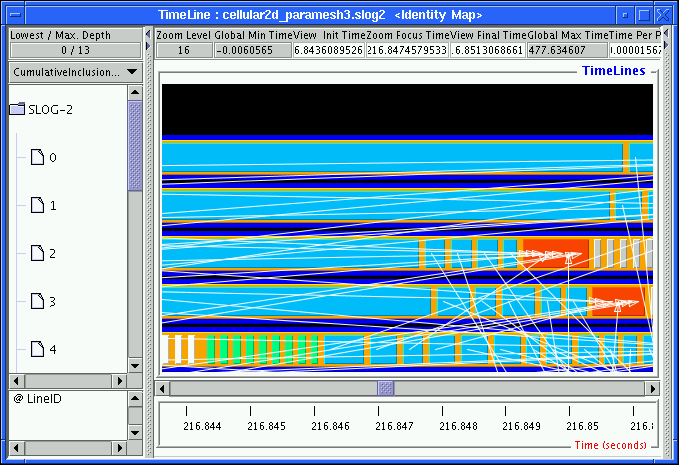
\includegraphics[%
  scale=0.6]{pic/timeline_preview_detail_4.png}


\caption{\label{fig:timeline_preview_detail_4} The next zoom-in view of Figure
\ref{fig:timeline_preview_detail_3}.}
\end{figure}



\chapter{Graphical User Interface}


\section{Main Window}

%
\begin{figure}[hbp]
\centering
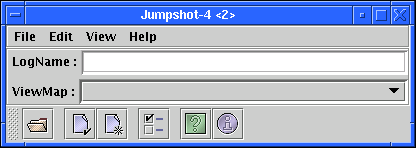
\includegraphics[%
  scale=0.6]{pic/main.png}


\caption{\label{fig:main} The main control window of Jumpshot-4.}
\end{figure}


The first window that pops up when inovking Jumpshot-4 is called Main
window as shown in Figure \ref{fig:main}. The buttons shown in toolbar
are shortcuts to the sub menu items in the top menubar. The function
of each of these buttons is listed in the Table \ref{table:main_toolbar}.
There are 2 textfields that display crucial information about the
logfile being processed. The textfield which is titled \emph{LogName}
displays the pathname of the SLOG-2 file being processed. The combobox
which is titled \emph{ViewMap} lists all the available ViewMaps in
the logfile. Currently, both CLOG%
\footnote{a low-overhead native trace format from MPE.%
} and RLOG%
\footnote{an internal MPICH2 profiling format%
} converted SLOG-2 file contains one ViewMaps, it is called the Identity
Map. Only IBM's UTE trace converted SLOG-2 file contains multiple
ViewMaps.

%
\begin{table}[hbp]
\begin{longtable}{|c|c|c|}
\hline 
Icon&
Description&
Function\tabularnewline
\hline
\hline 

\includegraphics[%
  scale=0.8]{pic/gif2png/Open24.png}&
File Selection &
display a File Chooser dialog to select logfile to be processed\tabularnewline
\hline 

\includegraphics[%
  scale=0.8]{pic/gif2png/Properties24.png}&
Show Legend Window&
display the Legend window of the selected logfile if it is hidden\tabularnewline
\hline 

\includegraphics[%
  scale=0.8]{pic/gif2png/New24.png}&
Show Timeline Window&
display the Timeline window of the selected logfile if it is hidden\tabularnewline
\hline 

\includegraphics[%
  scale=0.8]{pic/gif2png/Preferences24.png}&
Edit Preferences&
display the Preference window that adjusts Jumpshot's properties\tabularnewline
\hline 

\includegraphics[%
  scale=0.8]{pic/gif2png/Help24.png}&
Show User's Manual&
show the User's Manual of this program\tabularnewline
\hline

\includegraphics[%
  scale=0.8]{pic/gif2png/Information24.png}&
Show FAQs&
show the FAQs of this program\tabularnewline
\hline
\end{longtable}


\caption{\label{table:main_toolbar} Functions of the toolbar buttons}
\end{table}



\section{Legend Window}

As soon as a SLOG-2 file is selected in Main window, the Legend window
like the one shown in Figure \ref{fig:legend_popup} will be displayed. 

%
\begin{figure}[hbp]
\centering
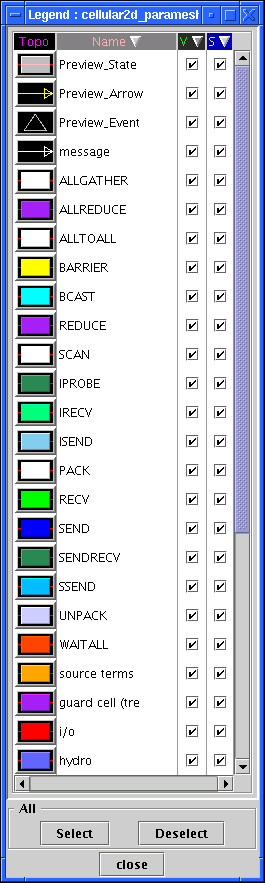
\includegraphics[%
  scale=0.6]{pic/legend_popup.png}


\caption{\label{fig:legend_popup} A typical Legend window when slog2 file
is first loaded into Jumpshot-4.}
\end{figure}


The Legend window contains mainly the 4 columns legend table. The
4 columns are labeled as \emph{Topo, Name, V} and \emph{S} as in Table
\ref{table:legend_column_ops}.

%
\begin{table}[hbp]
\begin{longtable}{|c|c|>{\centering}p{2in}|>{\centering}m{2in}|}
\hline 
\multicolumn{1}{|c|}{Icon}&
Description&
Left Mouse Click on Column Cell&
Right Mouse Click on Column Cell or Left Mouse Click on Column Title\tabularnewline
\hline
\hline 

\includegraphics[%
  scale=0.8]{pic/legend_topo.png}&
Topology&
Pick new Color (Figure \ref{fig:legend_color_chooser})&
None\tabularnewline
\hline 

\includegraphics[%
  scale=0.8]{pic/legend_name.png}&
Name&
Edit Name&
Sort Order menu (Figure \ref{fig:legend_sort_order})\tabularnewline
\hline 

\includegraphics[%
  scale=0.8]{pic/legend_v.png}&
Visibility&
Check or Uncheck&
Checkbox Operations Menu (Figure \ref{fig:legend_checkbox_ops})\tabularnewline
\hline 

\includegraphics[%
  scale=0.8]{pic/legend_s.png}&
Searchability&
Check or Uncheck&
Checkbox Operations Menu (Figure \ref{fig:legend_checkbox_ops})\tabularnewline
\hline
\end{longtable}


\caption{\label{table:legend_column_ops} Operations on the Legend window's
columns.}
\end{table}


Table \ref{table:legend_column_ops} also lists out all defined mouse
operations that are provided in each column. The operations are left
mouse clicking on the column title icon and on the column cell as
well as right mouse clicking in any column cell. 

%
\begin{figure}[hbp]
\centering
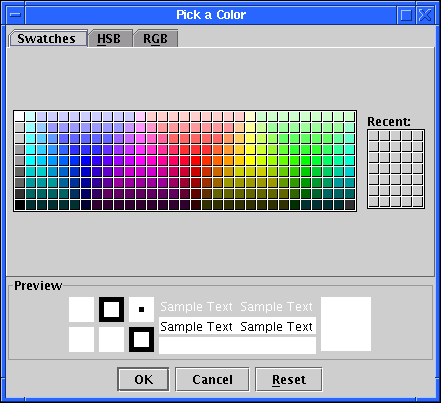
\includegraphics[%
  scale=0.6]{pic/legend_color_chooser.png}


\caption{\label{fig:legend_color_chooser} Color Chooser Dialog for column
Category Topology}
\end{figure}


Figure \ref{fig:legend_color_chooser} is the Color Chooser dialog
that will pop up when one of the icon buttons in column Topo is pressed.
The color editor provides 3 different ways of choosing a new color.
After selecting a new color from the dialog, the new color will be
used to update the icon button. The update won't be carried out in
the timeline canvas automatically, explicit screen redraw is needed.

%
\begin{figure}[hbp]
\centering
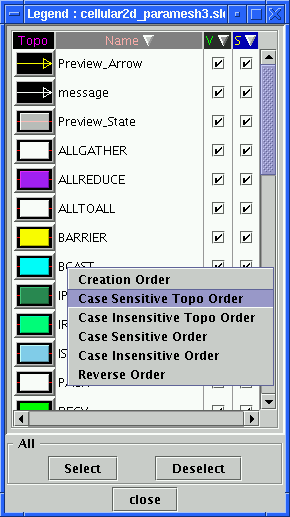
\includegraphics[%
  scale=0.6]{pic/legend_sort_menu.png}


\caption{\label{fig:legend_sort_order} Sort Order operation menu for the
column Category Name in the Legend window.}
\end{figure}


Figure \ref{fig:legend_sort_order} shows the popup dialog box either
when the title icon of column Name is pressed or when right mouse
button is clicked somewhere in the column. There are altogether 6
different sort orders. The first order in the list is called \emph{Creation
Order} which refers to the category order is stored in slog2 file
when it is being created. The 4 alphabetical ordering has a hidden
sort order that is not mentioned in their names. This hidden order
is called \emph{Preview Order} which puts the preview drawable category
before all the real drawable categories of the same topology. The
word \emph{Topo Order} refers to topologyical order. Taking altogether,
{}``Case Sensitive Topo Order'' means first topological order, preview
order, then case sensitive alphabetical order. The various orderings
serve to facilitate the continuous selection of the category rows
in the legend table. 

%
\begin{figure}[hbp]
\centering
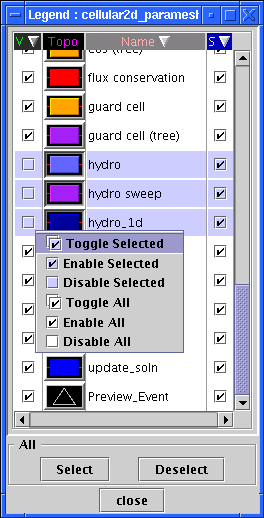
\includegraphics[%
  scale=0.6]{pic/legend_checkbox_menu.png}


\caption{\label{fig:legend_checkbox_ops} Checkbox Operation menu for column
Category Visibility and Searchability }
\end{figure}


Figure \ref{fig:legend_checkbox_ops} shows a popup dialog box when
the title icon of column V (Visibililty) or S (Searchability) is pressed
or when right mouse button is clicked somewhere in either columns.
The rule of selection in the legend table follows the standard practice
of other graphical user interfaces as in the Table \ref{table:selection_rules}.
Together with this standard selection rules, the operations provided
in checkbox operation menu allow easy enabling and disabling of visibility
as well as searchability checkboxes.

%
\begin{table}[hbp]
\begin{longtable}{|c|>{\centering}m{4in}|}
\hline 
Left Mouse Operation&
Action\tabularnewline
\hline
\hline 
\noun{Click}&
\emph{Click} on an object deselects any existing selection and selects
the object.\tabularnewline
\hline 
\noun{Control-Click}&
\emph{Control-click} on an object toggles its selection without affecting
the selection of any other objects\tabularnewline
\hline 
\noun{Shift-Click}&
\emph{Shift-click} on an object extends the selection from the most
recently selected object to the current object.\tabularnewline
\hline 
\noun{Dragging }&
\emph{Dragging} (that is, moving the mouse while holding down left
mouse button) through a range of \noun{text} deselects any existing
selection and selects the range of text.\tabularnewline
\hline
\end{longtable}


\caption{\label{table:selection_rules} Standard Selection Rules.}
\end{table}


\noun{NOTE:} Any changes done in the Legend window that alters the
appearance of drawables won't be automatically updated in the timeline
canvas until the CanvasReDraw button in the Timeline window is pressed.


\section{Timeline Window}

%
\begin{figure}[hbp]
\centering
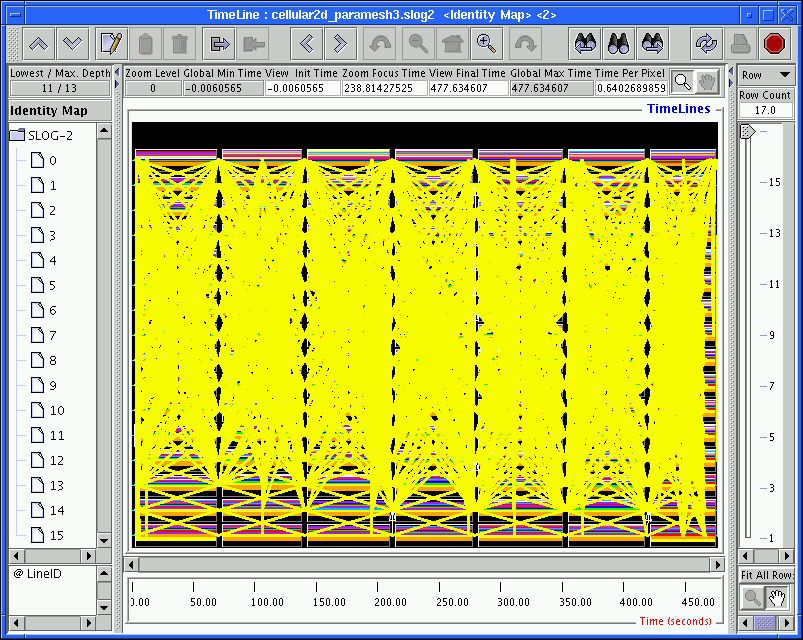
\includegraphics[%
  scale=0.6]{pic/timeline_popup.png}


\caption{\label{fig:timeline_popup} The initial display of the Timeline window
of a 506 MB 16 processes slog2 file with default preview resolution.}
\end{figure}


Figure \ref{fig:timeline_popup} is the initial display of the Timeline
window of a big 16 timelines slog2 file. Several concealable and removable
components are used to create the Timeline window. In the center of
the window, there is the \emph{timeline canvas}. Directly on top of
the timeline canvas is the \emph{time display panel}. On top of the
display panel, there is the removable \emph{toolbar}. To the left
of the canvas is the concealable \emph{Y-axis label panel}. To the
right of the canvas is the concealable \emph{row adjustment panel}.
At the bottom of the canvas is the \emph{time ruler canvas}. Both
Y-axis label and the row adjustment panels can be put out of sight
by clicking the tabs in the dividers or dragging the dividers. The
top toolbar can be dragged out of the window or be repositioned in
the other 3 sides of the window. After removal of the toolbar and
hidding of the left and right panels, the bare minimal Timeline window
looks like the one shown in Figure \ref{fig:timeline_preview_detail_0}. 


\subsection{Zoomable and Scrollable Canvas\label{sub:Zoomable-and-Scrollable}}

When viewing a big slog2 file like the one shown in Figure \ref{fig:timeline_popup},
the whole timeline canvas is filled up with preview drawables. Though
it provides a reasonable description at high level, i.e. one still
gets a vague sense where the long and/or frequent drawables are. Nevertheless,
it is pretty obscure to know the details. Hence, a well-designed zoomable
and scrollable user interface (ZSUI) of the timeline canvas becomes
an absolute necessity to facilitate the location of events of interest.
The ZSUI of the timeline canvas includes many parts and operations.
But the most handy ones are \emph{dragged zoom}, \emph{grasp and scroll}
and \emph{instant zoom in and out.}All these features are supported
by the Zoomable and Scrollable canvas. There are 2 such canvases in
the Timeline window. They are \emph{Timeline Canvas} and \emph{Time
Ruler Canvas}. In these canvases, left mouse clicking can be alternated
in 2 different modes by a pair of toggled buttons as shown in Figures
\ref{fig:mouse_zoom_mode} and \ref{fig:mouse_hand_mode}. They are
called \emph{Zoom} and \emph{Hand} modes. Each canvas in the Timeline
window has its own set of toggled buttons that determine its left
mouse click behavior. The timeline canvas's toggled buttons are located
above the canvas and sit at the end of the time display panel. The
time ruler's toggled buttons are located at the bottom of row adjustment
panel, i.e. sit right next to the end of the ruler. By default, the
timeline canvas is in zoom mode and the time ruler canvas is in hand
mode, so user can do zooming when the cursor is in the timeline canvas
and can scroll easily by simply moving the cursor over the ruler canvas.
Also, the scrolling can be done by simply dragging on scrollbar's
knob, clicking the end buttons and in the space between the knob and
scrollbar's end buttons.

%
\begin{figure}[hbp]
\centering

\includegraphics{pic/mouse_zoom_mode.png}


\caption{\label{fig:mouse_zoom_mode} Canvas's left mouse click is in zoom
mode.}
\end{figure}


%
\begin{figure}[hbp]
\centering

\includegraphics{pic/mouse_hand_mode.png}


\caption{\label{fig:mouse_hand_mode} Canvas's left mouse click is in hand
mode.}
\end{figure}



\subsubsection{Dragged Zoom}

%
\begin{figure}[hbp]
\centering

\includegraphics{pic/gif2png/ZoomPlusUpLeft25.png}


\caption{\label{fig:zoom_plus_cursor} Zoom-plus cursor that indicates the
left mouse clicking is ready for zooming in.}
\end{figure}


\emph{Dragged zoom} is active only when the left mouse click is in
zoom mode, i.e. when the the magnifying glass button is pressed in
the toggled buttons as in Figure \ref{fig:mouse_zoom_mode}. In zoom
mode, the cursor within the canvas will appear like a magnifying glass
with plus sign in the center as in Figure \ref{fig:zoom_plus_cursor}.
It is called zoom-plus cursor. The dragged zoom operation is initialized
by pressing the left mouse button at the beginning of the zoom-in
region, a white line will then appear. As soon as dragging is detected,
another white line will appear to mark the current ending of the zoom-in
region. The region that is marked by pair of white lines is lightly
shaded as shown in Figure \ref{fig:timeline_preview_detail_3}. The
process can be cancelled anytime by hitting the ESC key during dragging.
Once the left mouse button is released, zooming will be carried out
and the Timeline window will then be updated as in Figure \ref{fig:timeline_preview_detail_4}.
The time display panel is updated with the latest time related information
of the zoom-in region. Notice that the zooming as well as scrolling
can be achieved by explicitly editing the text fields in the time
display panel.


\subsubsection{Instant Zoom}

%
\begin{figure}[hbp]
\centering

\includegraphics{pic/gif2png/ZoomMinusUpLeft25.png}


\caption{\label{fig:zoom_minus_cursor} Zoom-minus cursor that indicates the
left mouse clicking is ready for zooming out.}
\end{figure}


While the canvas is still in zoom mode, \emph{instant zoom} is enabled
by default. Instant zoom allows zooming in at the point of left mouse
clicking by a factor of 1/2, i.e. the region centered at the point
of left clicking will be magnified by a factor or 2. Also, the \emph{Zoom
Focus Time} in the time display panel will be updated with the time
where left clicking on the canvas is detected. In the process, the
cursor remain\emph{s} zoom-plus cursor. \emph{Shift-click}, on the
other hand, will do the opposite. While holding down Shift key, the
cursor will be changed to a zoom-minus cursor as in Figure \ref{fig:zoom_minus_cursor}
to indicate zooming out is the action associated with left clicking.
The zoom factor is 2 in this case.


\subsubsection{Grasp and Scroll}

%
\begin{figure}[hbp]
\centering

\includegraphics{pic/gif2png/HandOpenUpLeft25.png}


\caption{\label{fig:hand_open_cursor} Open hand cursor indicates that left
mouse clicking is ready to grasp and scroll.}
\end{figure}


%
\begin{figure}[hbp]
\centering

\includegraphics{pic/gif2png/HandCloseUpLeft25.png}


\caption{\label{fig:hand_close_cursor} Close hand cursor indicates that left
mouse clicking is scrolling.}
\end{figure}


\emph{Grasp and Scroll} is active only when the left mouse click is
in hand mode, i.e. when the open hand button is pressed as in Figure
\ref{fig:mouse_hand_mode}. The cursor in hand mode is an open hand
as in Figure \ref{fig:hand_open_cursor}. As soon as left mouse button
is pressed down, the cursor turns to a close hand as in Figure \ref{fig:hand_close_cursor}.
It indicates the canvas will move in the same direction that the cursor
moves as long as the left mouse button remain pressed. The grasp and
scroll mode in time ruler canvas can only move horizontally, but the
grasp and scroll mode in timeline canvas allows movement in both vertical
and horizontal axes. 


\subsubsection{Information Dialog Box}

Jumpshot-4 wouldn't be complete if it cannot provide a way to tell
user what exactly are being displayed. It is particularly important
when there are many preview drawables. Following standard user interface
practice, Jumpshot-4 uses \emph{right mouse clicking} as an interface
for user to tell Jumpshot-4 what object that more information is needed.
In general, anywhere on the canvas, both timeline and time ruler canvases,
can be inquired with right mouse clicks. Information dialog box will
pop up accordingly to tell user more about object that is being clicked.
There are 3 different types of information dialogs: Drawable Info
Box, Duration Info Box and Time Info Box. All these info boxes remain
in memory as long as they are not closed even if the canvas has been
scrolled or zoomed. One of the usages of the info boxes is to serve
as time markers in between zooming and scrolling.


\paragraph{Drawable Info Box}

Drawable Info Box is a popup dialog box that provides detailed information
about the drawable object that is being clicked. There are 2 different
kind of Drawable Info Box, one for preview drawable, one for real
drawable. 


\subparagraph{Drawable Info Box for Preview Drawable}

%
\begin{figure}[hbp]
\centering

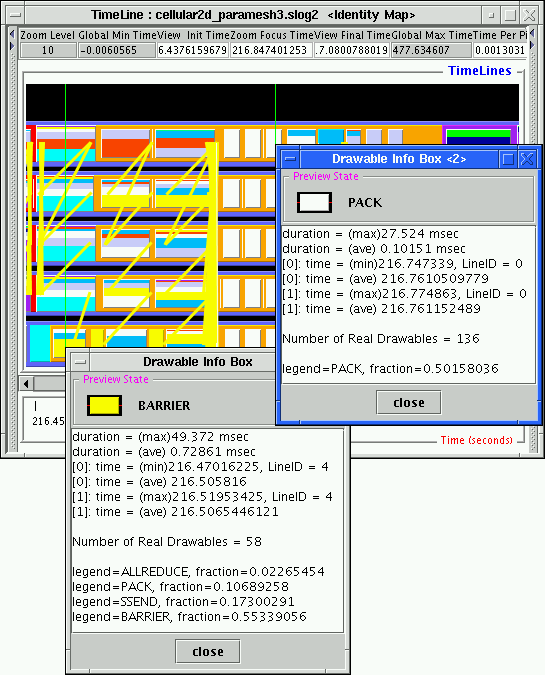
\includegraphics[%
  scale=0.6]{pic/timeline_infobox_preview_state.png}


\caption{\label{fig:timeline_infobox_preview_state} Drawable Info Box for
Preview State}
\end{figure}


Right mouse clicking on 2 of the preview states in the timeline canvas
shown in Figure \ref{fig:timeline_preview_detail_1} will pop up 2
Drawable Info Boxes for the preview states. They are displayed as
in Figure \ref{fig:timeline_infobox_preview_state}. The popup Info
Box's upper left hand corner will be positioned at exactly where right
mouse click is detected and a green line marker is drawn on the canvas
to indicate what time has been clicked in case the dialog box is moved
from its original popup location. In order to best illustrate what
information is presented by the Drawable Info Box, let's take the
highlighted Drawable Info Box in Figure \ref{fig:timeline_infobox_preview_state}
as an example. The dialog box which contains a pink label {}``Preview
State'' is the Drawable Info Box for preview state, and the icon
inside the dialog box shows the color and shape that are used to draw
the drawable. Below the icon, there is a big text area that prints
all the detailed statistical information about this preview state.
There are 6 timestamps in the text area: maximum duration, average
duration, minimum starttime, average starttime, maximum endtime and
average endtime. Here {}``{[}0{]}'' refers to starting point, and
{}``{[}1{]}'' refers to the ending point. The 3 {}``average''
timestamps are averaged over all the real drawables represented by
this preview drawable. Besides timestamps, the info box also tells
{}``Number of Real Drawables'' represented by the preview object.
In this case, 136 real states are amalgamated by the pure white preview
state. Also, the text area lists all the different categories of drawables
amalgamated and their ratios of the cumulative duration of all real
drawables amalgamated to the duration the preview states. In this
case, there is only 1 category of real states in this preview state,
so all 136 states are all PACKs. The sum of the durations of all PACKs
is about half of the duration of the preview state as it is indicated
by {}``fraction=0.50158036'' which is called category weight. 

Another Drawable Info Box is shown at the lower portion of Figure
\ref{fig:timeline_infobox_preview_state}. Here the preview state
that is pointed by the upper left-hand corner of the Info Box has
3 different strips of colors: yellow, royal blue and white. Right
mouse clicking at the yellow strip pops up a Drawable Info Box with
a yellow state icon with label BARRIER. As shown in the figure, this
preview state amalgmated 4 different categories of real states: ALLREDUCE,
PACK, SSEND, and BARRIER. The statistically most significant one is
BARRIER which proportionally occupies 0.55339056 of the length of
the preview state. Hence BARRIER strip has the tallest height among
all the color strips shown in the preview state. Clicking on the different
color strip in the same preview state will pop up a Drawable Info
Box that has a different icon label of with corresponding color, but
the content of the text area should remain the same. Out of the 4
categories mentioned in the text area, only 3 are graphically displayed
in the figure given the limited pixel height availabel to the preview
state. The least significant category ALLREDUCE is missing visually.
But the limitation can be improved by selecting another display option
for preview state in Preference window that does not rely on the category
weight%
\footnote{i.e. by setting the PREVIEW\_STATE\_DISPLAY in Preference window to
MOST\_LEGENDS\_ORDER as listed in Table \ref{table:preference_data2} %
}. As indicated, there are 58 real drawables in the preview state,
but no information is provided about how many real drawables are in
each real categories.


\subparagraph{Drawable Info Box for Real Drawable}

%
\begin{figure}[hbp]
\centering
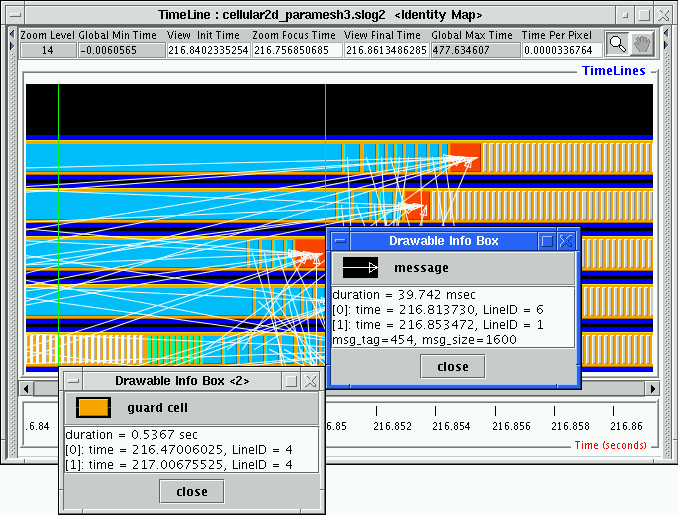
\includegraphics[%
  scale=0.6]{pic/timeline_infobox_real_primitive.png}


\caption{\label{fig:timeline_infobox_real_primitive} Drawable Info Box for
real state and arrow. The Drawable Info Box for the arrow shows the
messsage size, 1600 byte, and tag ID, 454.}
\end{figure}


Similarly for real drawables, Drawable Info Box can be brought up
by right mouse clicking on the real drawables. In Figure \ref{fig:timeline_infobox_real_primitive},
Drawable Info Boxes for a real arrow and a real state are shown. The
Drawable Info Box for the arrow is invoked by clicking anywhere within
the vicinity of the arrow body%
\footnote{The vincinity width can be adjusted by modifying the parameter CLICK\_RADIUS\_TO\_LINE
in Preference window as listed in Table \ref{table:preference_data1}.
The default is 3 pixels.%
}, and the info box shows the starttime, start timeline ID, endtime,
and ending timeline ID and some extra information implemented by the
native format . In this example, the message size carried by the specific
arrow is 1600 byte.


\paragraph{Duration Info Box}

%
\begin{figure}[hbp]
\centering
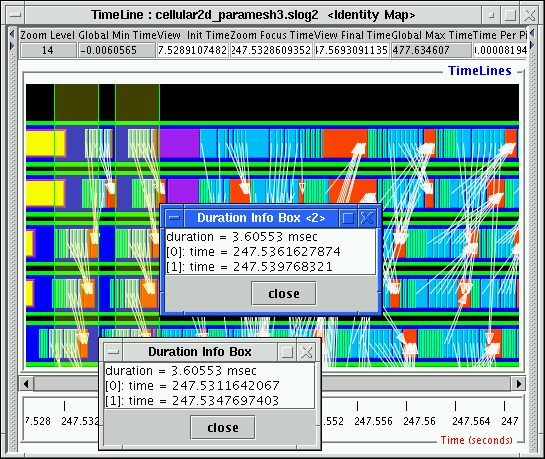
\includegraphics[%
  scale=0.6]{pic/timeline_infobox_duration.png}


\caption{\label{fig:timeline_infobox_duration} Duration Info Box shows the
duration, starttime, and endtime of a time region marked by a pair
of green lines.}
\end{figure}


Duration Info Box is created by right dragging a region of empty space
in the timeline canvas or the time ruler canvas. The dragged region
will be marked by a pair of green lines and is lightly shaded as well.
One of the usages of Duration Info Box is to compare different durations
to see if they are the same. For instance in Figure \ref{fig:timeline_infobox_duration},
the 2 Duration Info Boxes mark 2 non-overlap regions on the 3rd timeline
to check if the total duration taken up by the all consecutive small
states within the 2 regions are the same. As shown in the Duration
Info Box, it appears the total durations are the same. 


\paragraph{Time Info Box}

%
\begin{figure}[hbp]
\centering
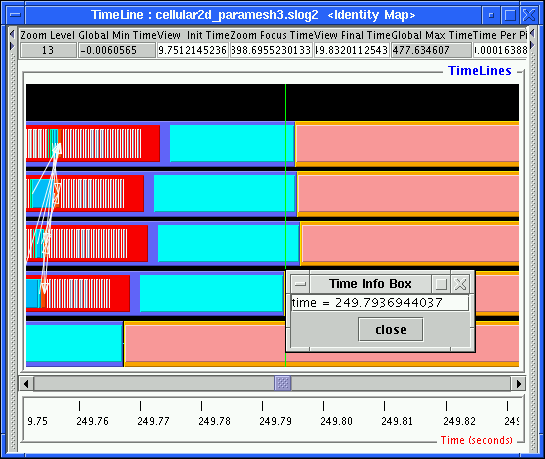
\includegraphics[%
  scale=0.6]{pic/timeline_infobox_time.png}


\caption{\label{fig:timeline_infobox_time} Time Info Box displays the time
of where it pops up.}
\end{figure}


Time Info Box is created by right clicking in the empty space in either
timeline or tthe time ruler canvas as in Figure \ref{fig:timeline_infobox_time}.
This Info Box is usually used as a marker for a single event in time.


\subsection{Toolbar}

The buttons in the toolbar of Timeline window provides various basic
services to the Timeline window. Table \ref{table:timeline_toolbar}
contains the list of functionalities of the buttons found in the toolbar.

%
\begin{table}[hbp]
\begin{longtable}{|c|c|c|>{\centering}m{3.5in}|}
\hline 
Icon&
Description&
Shortcut&
Function\tabularnewline
\hline
\hline 

\includegraphics[%
  scale=0.8]{pic/gif2png/Up24.png}&
Up&
Alt-UP&
Scroll upward by half a screen\tabularnewline
\hline 

\includegraphics[%
  scale=0.8]{pic/gif2png/Down24.png}&
Down&
Alt-DOWN&
Scroll downward by half of a screen\tabularnewline
\hline 

\includegraphics[%
  scale=0.8]{pic/gif2png/Edit24.png}&
LabelMark&
none&
Mark the timeline(s)\tabularnewline
\hline 

\includegraphics[%
  scale=0.8]{pic/gif2png/Paste24.png}&
LabelMove&
none&
Move the marked timeline(s)\tabularnewline
\hline 

\includegraphics[%
  scale=0.8]{pic/gif2png/Delete24.png}&
LabelDelete&
none&
Delete the marked timeline(s)\tabularnewline
\hline 

\includegraphics[%
  scale=0.8]{pic/gif2png/TreeExpand24.png}&
LabelExpand&
Alt-E&
Expand the Y-axis tree label by 1 level\tabularnewline
\hline 

\includegraphics[%
  scale=0.8]{pic/gif2png/TreeCollapse24.png}&
LabelCollapse&
Alt-C&
Collapse the Y-axis tree label by 1 level\tabularnewline
\hline 

\includegraphics[%
  scale=0.8]{pic/gif2png/Backward24.png}&
Backward&
Alt-LEFT&
Scroll Backward by half a screen\tabularnewline
\hline 

\includegraphics[%
  scale=0.8]{pic/gif2png/Forward24.png}&
Forward&
Alt-RIGHT&
Scroll Forward by half a screen\tabularnewline
\hline 

\includegraphics[%
  scale=0.8]{pic/gif2png/WinUndo.png}&
ZoomUndo&
Alt-U&
Undo the previous zoom operation\tabularnewline
\hline 

\includegraphics[%
  scale=0.8]{pic/gif2png/ZoomOut24.png}&
ZoomOut&
Alt-O&
Zoom Out by 1 level in time\tabularnewline
\hline 

\includegraphics[%
  scale=0.8]{pic/gif2png/Home24.png}&
ZoomHome&
Alt-H&
Reset zoom to the initial resolution in time\tabularnewline
\hline 

\includegraphics[%
  scale=0.8]{pic/gif2png/ZoomIn24.png}&
ZoomIn&
Alt-I&
Zoom In by 1 level in time\tabularnewline
\hline 

\includegraphics[%
  scale=0.8]{pic/gif2png/WinRedo.png}&
ZoomRedo&
Alt-R&
Redo the previous zoom operation\tabularnewline
\hline 

\includegraphics[%
  scale=0.8]{pic/gif2png/FindBack24.png}&
SearchBackward&
Alt-B&
Search backward in time\tabularnewline
\hline 

\includegraphics[%
  scale=0.8]{pic/gif2png/Find24.png}&
SeachInitialize&
Alt-S&
Search Initialization from last popup InfoBox's time\tabularnewline
\hline 

\includegraphics[%
  scale=0.8]{pic/gif2png/FindFore24.png}&
SearchForward&
Alt-F&
Search forward in time\tabularnewline
\hline 

\includegraphics[%
  scale=0.8]{pic/gif2png/Refresh24.png}&
CanvasReDraw&
Alt-D&
Redraw canvas to synchronize changes from Preference/Legend window
or Yaxis label panel.\tabularnewline
\hline 

\includegraphics[%
  scale=0.8]{pic/gif2png/Print24.png}&
Print&
none&
Print the Timeline window\tabularnewline
\hline 
\includegraphics[%
  scale=0.8]{pic/gif2png/Stop24.png}&
Exit&
none&
Exit the Timeline window\tabularnewline
\hline
\end{longtable}


\caption{\label{table:timeline_toolbar} Table of toolbar's functionalities.}
\end{table}



\subsection{Y-axis Label Panel}

The concealable left panel in Timeline window is called Y-axis label
panel which contains a tree-like representation for Y-axis label for
the timelines. For a single viewmaps slog2 file from CLOG or RLOG,
the typical Y axis label panel looks like that is shown in Figure
\ref{fig:yaxis_label_panel_simple}. Together with toolbar's label
buttons, e.g. LabelMark and LabelMove, and standard selection methods
by mouse click listed in Table \ref{table:selection_rules}, labels
can be rearranged easily to create a more easily understood timeline
canvas. For multiple viewmaps slog2 from IBM's UTE trace enviroment,
LabelExpand and LabelCollapse buttons will come in handy to expand
and collapse the label tree by one whole level. In order to minimize
unnecessary redraw of the timeline canvas, the sychronization between
the label panel and the timeline canvas is carried out passively,
i.e. user needs to press the CanvasReDraw button in the toolbar to
update the Timeline window with the changes from the label panel.

%
\begin{figure}[hbp]
\centering
\includegraphics[%
  scale=0.6]{pic/yaxis_label_panel_simple.png}


\caption{\label{fig:yaxis_label_panel_simple} A simple 1 level Yaxis label
tree. The highlighted labels are those that have been selected.}
\end{figure}



\subsection{Row Adjustment Panel}

The concealable right panel in Timeline window contains the row adjustment
panel which is used to determine the row adjustment scheme. There
are 2 different modes in row adjustment panel: row count mode and
row height mode. These 2 modes can be selected by the combox at the
top of the panel. The row count mode attemps to keep the number of
timelines constant as indicated in the Row Count text field when the
Timeline window resizes. On the other hand, the row height mode fixes
the height of each timeline as indicated by the Row Height text field.
Currently, the height of the timeline can be adjusted up to the height
of the timeline canvas, in that case the Row Count text field shows
a number 1%
\footnote{If the slog2 file contains numerous timelines, increasing the Row
Height will increase the size of the images managed by Jumpshot-4.
This may cause the Java Virtual Machine to exhaust all its memory
if the virtual machine is not set to have enough memory when Jumpshot-4
is started or there isn't enough physical memory in machine that Jumpshot-4
runs on. %
}. The maximum number of timelines that can be displayed is set to
the total number of rows represented by the whole Y-axis label tree%
\footnote{Hence the row height cannot be adjusted all the way to zero.%
}. For multiple viewmaps slog2 file, the Y-axis label tree can be expanded
or collapsed. This could change the maximum number of rows in the
row count slider after user hits the CanvasReDraw button. Coupling
with window resize, the row adjustment panel allows user to magnify
or shrink the height of the timeline as one desires.

%
\begin{figure}[hbp]
\centering
\subfigure[Row Count mode]{\includegraphics[%
  scale=0.6]{pic/adj_row_count.png}}~~~~~~~~~~~~~~~\subfigure[Row Height mode]{\includegraphics[%
  scale=0.6]{pic/adj_row_height.png}}


\caption{\label{fig:row_adjustment_panel} Row Adjustmemt Panel determines
the Timeline window's resize scheme. When one of the mode sliders
or textfields is adjusted, the other 3 components will be adjusted
simultaneously.}
\end{figure}



\section{Preference Window}

%
\begin{figure}[hbp]
\centering
\includegraphics[%
  scale=0.6]{pic/preference_pview_state.png}


\caption{\label{fig:preference_pview_state} The Preference window that shows
PREVIEW\_STATE\_DISPLAY}
\end{figure}


As shown in Figure \ref{fig:preference_pview_state} is the Preference
window that adjusts the various display properties of the visualization
program. A list of the parameters and their definitions are listed
in Tables \ref{table:preference_data1} and \ref{table:preference_data2}.

%
\begin{table}[hbp]
\centering
\begin{longtable}{|c|p{1.1in}|p{3.5in}|}
\hline 
Parameter&
Values&
Description\tabularnewline
\hline
\hline 
{\small Y\_AXIS\_ROOT\_LABEL}&
any text&
Label for the root node of the Y-axis tree label in the left panel.\tabularnewline
\hline 
INIT\_SLOG2\_LEVEL\_READ&
+ve integer&
The number of slog2 levels being read into memory when the Timeline
window is initialized, the integer affects the zooming and scrolling
performance exponentially (in a asymptotical sense).\tabularnewline
\hline 
AUTO\_WINDOWS\_LOCATION&
true, false&
Whelther to let Jumpshot-4 automatically set windows placement\tabularnewline
\hline 
SCREEN\_HEIGHT\_RATIO&
0.0 ... 1.0&
Ratio of the initial timeline canvas height to the screen height\tabularnewline
\hline 
TIME\_SCROLL\_UNIT\_RATIO&
0.0 ... 1.0&
Unit increment of the horizontal scrollbar in the fraction of timeline
canvas's wdith.\tabularnewline
\hline 
Y\_AXIS\_ROOT\_VISIBLE&
true, false&
Whelther to show the top of the Y-axis tree-styled directory label.\tabularnewline
\hline 
BACKGROUND\_COLOR&
Black, DarkGray, Gray, LightGray, White&
Background color of the timeline canvas\tabularnewline
\hline 
ACTIVE\_REFRESH&
false&
Whelther to let Jumpshot-4 actively update the timeline canvas.\tabularnewline
\hline 
STATE\_BORDER&
ColorRaised, ColorLowered, WhiteRaised, WhiteLowered, WhitePlain,
Empty&
Border style of real states.\tabularnewline
\hline 
STATE\_HEIGHT\_FACTOR&
0.0 ... 1.0&
Ratio of the outermost rectangle height to row height. The larger
the factor is, the larger the outermost rectangle will be with respect
to the row height.\tabularnewline
\hline 
NESTING\_HEIGHT\_FACTOR&
0.0 ... 1.0 &
The gap ratio between successive nesting rectangles. The larger the
factor is, the smaller the gap will be.\tabularnewline
\hline 
ARROW\_ANTIALIASING&
default, on, off&
Whelther to draw arrow with anti-aliasing lines. Turning this on will
slow down the canvas drawing by a factor of 3.\tabularnewline
\hline 
ARROW\_HEAD\_LENGTH&
+ve integer&
Length of arrow head in pixel.\tabularnewline
\hline 
ARROW\_HEAD\_HALF\_WIDTH&
+ve integer&
Half width of arrow head's base in pixel.\tabularnewline
\hline 
CLICK\_RADIUS\_TO\_LINE&
+ve integer&
Radius in pixel for a click to be considered on the arrow.\tabularnewline
\hline
\end{longtable}


\caption{\label{table:preference_data1} Modifiable parameters in Preference
window. }
\end{table}


%
\begin{table}[hbp]
\centering
\begin{longtable}{|c|p{1.1in}|p{3.5in}|}
\hline 
Parameter&
Values&
Description\tabularnewline
\hline
\hline 
PREVIEW\_STATE\_DISPLAY&
DecreLegendOrder, DecreWeightOrder, MostLegndsOrder&
Display option of Preview state.\tabularnewline
\hline 
PREVIEW\_STATE\_BORDER&
ColorRaised, ColorLowered, WhiteRaised, WhiteLowered, WhitePlain,
Empty&
Border style of Preview state.\tabularnewline
\hline 
PREVIEW\_STATE\_LEGEND\_H&
integer&
Minimum height of the legend divison in pixel for the Preview state\tabularnewline
\hline 
PREVIEW\_STATE\_BORDER\_W&
integer&
The empty border insets' width in pixel for the Preview state.\tabularnewline
\hline 
PREVIEW\_STATE\_BORDER\_H&
integer&
The empty border insets' height in pixel for the Preview state.\tabularnewline
\hline 
PREVIEW\_ARROW\_LINE\_W&
float&
The line thickness in pixel for the Preview arrow.\tabularnewline
\hline 
MIN\_WIDTH\_TO\_DRAG&
integer&
Minimum width in pixel to be considered a dragged operation.\tabularnewline
\hline 
SEARCH\_ARROW\_LENGTH&
integer&
Length of the search marker's arrow in pixel\tabularnewline
\hline 
SEARCH\_FRAME\_THICKNES&
integer&
Thickness in pixel of the popup frame that hightlights the searched
drawable\tabularnewline
\hline 
SEARCHED\_OBJECT\_ON\_TOP&
true, false&
Whelther to display the searched object on top of the search frame.\tabularnewline
\hline 
LEFTCLICK\_INSTANT\_ZOOM&
true, false&
Whelther to zoom in immediately after left mouse click on canvas.\tabularnewline
\hline
\end{longtable}


\caption{\label{table:preference_data2}Modifiable parameters in Preference
window}
\end{table}



\chapter{Special Features}


\section{Search and Scan Facility}

The Level-of-detail support provided in SLOG-2 and Jumpshot-4 tends
to help locate states which are either longer in time or occur very
frequently. States that are short and occur rarely in a big logfile
are very difficult to locate without any special tool. In Jumpshot-4,
a search and scan facility is provided to facilitate this goal. There
are 3 search criteria: search time, searchable timeline IDs and searchable
categories. 

\begin{enumerate}
\item \emph{Search Time} is the time that search starts. It is marked by
a yellow line calld search cursor. There are 2 differnt ways of setting
the search cursor. When the timeline canvas is in Hand mode as described
in Figure \ref{fig:mouse_hand_mode} of section \ref{sub:Zoomable-and-Scrollable},
left mouse clicking will set the search cursor. The other way can
be done in either Hand or Zoom mode. First popup an information dialog
box of any kind using right mouse clicking, then press the SearchInitialize
button in the toolbar to replace the green line by the yellow search
cursor. When there are more than one information dialog box, the information
dialog box that is shown up last will have its green line used to
initialize the search cursor. When Timeline window first starts up,
the search cursor is set at the starttime of the logfile.
\item \emph{Searchable Timeline IDs} are the timlines that search will operate
on, i.e only states on the marked timelines will be returned by the
search facility. These marked timelines can be selected by clicking
on their timeline IDs on Yaxis label panel with rules described in
Table \ref{table:selection_rules}. When nothing is selected, all
timelines are searchable.
\item \emph{Searchable Categories} are categories that have their searchable
checkboxes enabled as in Figure \ref{fig:legend_checkbox_ops}. Only
drawable with searchable category can be returned by the search facility.
By default, all categories in Legend window are searchable. 
\end{enumerate}
%
\begin{figure}[hbp]
\centering
\includegraphics[%
  scale=0.6]{pic/timeline_search_preview.png}


\caption{\label{fig:timeline_search_preview} Search of state \emph{eos} in
preview stage. The returned state is a preview state containing state
\emph{eos} as shown in Search Box and Drawable Info Box.}
\end{figure}


After setting any needed search criteria, the search operation can
be carried out by pressing either the SearchForeward or SearchBackward
buttons shown in the Table \ref{table:timeline_toolbar}. As shown
in Figure \ref{fig:timeline_search_preview}, the search facility
returns a searched state which is bounded by a 3D raised bordered
and transparent %
\footnote{the transparency of the 3D raised box can be made opaque by selecting
the SEARCHED\_OBJECT\_ON\_TOP true.%
}box whose starttime is marked by a yellow search cursor and 2 3D arrowheads.
The upper 3D arrow's color matches that of the returned state. In
the figure, since the returned state is a preview state, so the upper
3D arrow is grey in color as it is shown in Legend window. Accompanied
with the 3D raised bordered box is a popup Search Box that shows the
detailed of the preview state like the Drawable Info Box in Figure
\ref{fig:timeline_infobox_preview_state}. Since the search in the
figure is looking for state \emph{eos}, a Drawable Info Box is shown
to indicate the returned 3D bordered box does contain category \emph{eos}
graphically. In order to locate the real state \emph{eos}, a dragged
zoom is performed around the 3D raised bordered box and the result
is shown in Figure \ref{fig:timeline_search_preview_zoomed}. In the
figure, the real \emph{eos} is located at the end of the original
3D bordered box and it is marked by the Drawable Info Box.

%
\begin{figure}[hbp]
\centering
\includegraphics[%
  scale=0.6]{pic/timeline_search_preview_zoomed.png}


\caption{\label{fig:timeline_search_preview_zoomed} Dragged zoom the region
around the 3D raised bordered box in Figure \ref{fig:timeline_search_preview}
shows the real state \emph{eos.}}
\end{figure}


In general, when searching on big slog2 file, all preview categories
should be set searchable, otherwise searching for real drawables may
not return anything. Because at lower zoom level, there may not be
any real drawable belong to the categories of interest, only preview
drawable contains the categories of interest. Also, the search facility
is carried out for the drawables that are in the physical memory.
In some rare occasions, drawables in the memory may have been exhausted
for searching but end of the logfile have not been reached, user may
need to advance the search by scroll forward or backward to read in
more drawables and to restart the search again. For a very big logfile,
the search process of a real state may require repeated operations
of search and dragged zoom before the real state can be found. This
process will be automated in the later version of Jumpshot-4.


\section{Tuning of the Timeline Window}

%
\begin{figure}[hbp]
\centering
\includegraphics[%
  scale=0.6]{pic/timeline_popup_more.png}


\caption{\label{fig:timeline_popup_finer} The initial Timeline window with
finer preview resolution.}
\end{figure}


One of the major improvements in the new Jumpshot and SLOG-2 is the
scalability in terms of visualization performance. As shown in Figure
\ref{fig:timeline_popup}, there are 7 bands of preview states covering
the whole canvas in the initial Timeline window. By incrementing the
parameter, INIT\_SLOG2\_LEVEL\_READ, by 1 in Preference window as
in Table \ref{table:preference_data1}, the initial Timeline window
can be redisplayed and is shown in Figure \ref{fig:timeline_popup_finer}.
The new Timeline window has 14 bands of preview states instead of
7. The increase preview resolution does offer a more detailed description
of logfile but at the expense of graphical performance. Because every
increment of INIT\_SLOG2\_LEVEL\_READ will roughly double the number
of drawables to be iterated during every zooming or scrolling%
\footnote{it is true for a binary tree%
}. The biggest demand of graphical performance occurs when the zooming
to the level of only pure real drawables from the lower zoom level.
The value of INIT\_SLOG2\_LEVEL\_READ should be chosen so that Jumpshot
does not appear to be too slow during the zooming to the pure real
drawable level. For a fast graphics system, INIT\_SLOG2\_LEVEL\_READ
should be set higher than the default value 3, like 4 or 5, so that
more information is present during each view.

Another parameter also signifcantly affects the graphical performance
is ARROW\_ANTIALIASING in Preference window. Setting the paramters
to ON will force Jumpshot to draw all arrows including preview arrows
with anti-aliasing lines. This proves to be an expensive graphical
operation%
\footnote{A typical timeline canvas with arrows will draw roughly a factor 3
slower with anti-aliasing on. %
}. Except when high quality picture is needed like during screen capture
for picture or when antialiasing lines are drawn with graphics hardware
support, it is not recommended to turn on ARROW\_ANTIALIASING. 
\end{document}
